\documentclass[runningheads]{llncs}

\usepackage[T1]{fontenc}
\usepackage{graphicx}
\usepackage{amsmath}
\usepackage{amssymb}
\usepackage{booktabs}
\usepackage{multirow}
\usepackage[nocompress]{cite}
\usepackage{url}
\usepackage{xcolor}
\usepackage{array}

\newcolumntype{P}[1]{>{\centering\arraybackslash}p{#1}}

\begin{document}

\titlerunning{Long-Sequence Deep Unfolding for Limited-Angle CT}
\title{Benchmarking Long-Sequence Attention and State-Space Mechanisms in Deep Unfolding Networks for Limited-Angle CT Reconstruction}

\author{Dinh-Minh Phan\inst{1} \and 
Doanh C. Bui\inst{1} \and 
Khang Nguyen\inst{1}}

\authorrunning{D.-M. Phan et al.}

\institute{University of Information Technology, VNU-HCM, Ho Chi Minh City, Vietnam \\
\email{23520949@gm.uit.edu.vn, doanhbc@gm.uit.edu.vn, khangnttm@gm.uit.edu.vn}}

\maketitle

\begin{abstract}
Limited-angle computed tomography (LA-CT) is an ill-posed inverse problem that suffers from severe missing-wedge artifacts due to incomplete angular scanning geometries. Deep unfolding networks, which unroll iterative optimization algorithms into cascading neural stages, offer physics-guided reconstruction by interleaving data fidelity operations with learned regularization priors. However, conventional CNN-based regularizers suffer from restricted receptive fields that cannot resolve non-local geometric streak trajectories across the angular void, while standard Vision Transformers incur intractable $\mathcal{O}(N^2)$ quadratic computational complexity on high-resolution CT grids. In this work, we conduct a systematic empirical benchmark evaluating three emerging linear and sub-quadratic long-sequence modeling paradigms integrated as learnable regularizers within the LEARN unrolling framework: (1) sliding-window attention with global tokens (\textbf{Longformer}), (2) multi-scale exponentially dilated attention (\textbf{LongNet}), and (3) selective state-space sequential models (\textbf{Mamba}), benchmarked comprehensively against both the canonical CNN-based unrolling baseline (\textbf{LEARN}) and a dual-domain transformer architecture (\textbf{DuDoTrans}). 
Comprehensive experiments on the clinical Mayo Clinic Low-Dose CT (LDCT) benchmark across moderate ($120^\circ$) and severe ($90^\circ$) limited-angle regimes reveal critical architectural behaviors: (i) Under moderate $120^\circ$ scanning, \textbf{LEARN\_Longformer} attains superior reconstruction fidelity (33.10 dB PSNR and 0.0224 RMSE), outperforming canonical CNN LEARN (32.29 dB, +0.81 dB) and dual-domain DuDoTrans (25.15 dB, +7.95 dB), proving that localized windowing paired with sparse global anchors is optimal for non-local streak cancellation; (ii) \textbf{LEARN\_LongNet} delivers robust multi-scale artifact suppression (31.62 dB PSNR, 0.8991 SSIM); (iii) Under extreme $90^\circ$ truncation, dual-domain inpainting in \textbf{DuDoTrans} exhibits remarkable resilience (21.81 dB PSNR vs. 19.16 dB for Longformer), highlighting the benefit of projection-domain interpolation when first-order image gradients vanish in the Fourier void; and (iv) \textbf{LEARN\_Mamba} achieves 26.32 dB PSNR at $120^\circ$ but undergoes acute performance degradation under severe $90^\circ$ truncation (18.76 dB PSNR, 0.4292 SSIM), uncovering the structural vulnerability of 1D causal scanning when encountering 2D anisotropic frequency voids. Our findings provide foundational architectural guidelines for modern deep unrolling models in tomographic imaging.

\keywords{Limited-Angle CT \and Deep Unfolding \and Long-Sequence Modeling \and Transformer \and Longformer \and LongNet \and Mamba \and DuDoTrans \and Empirical Benchmark.}
\end{abstract}

\section{Introduction}
\label{sec:intro}

X-ray Computed Tomography (CT) is an indispensable non-invasive diagnostic modality in modern healthcare \cite{wang2020deep,kak2001principles}. However, in numerous specialized clinical and interventional scenarios---such as C-arm intraoperative imaging, dental tomosynthesis, and image-guided radiotherapy---physical mechanical clearance or scanning time constraints restrict the gantry's angular coverage to a limited angular range (e.g., $120^\circ$ or $90^\circ$ instead of the full $180^\circ$ or $360^\circ$) \cite{chen2018learn,sidky2008image}. This condition, known as Limited-Angle CT (LA-CT), represents a severely ill-posed inverse problem. According to the Fourier Slice Theorem \cite{kak2001principles}, incomplete angular sampling creates a non-sampled ``missing wedge'' in Fourier frequency space. Direct analytical inversion using Filtered Backprojection (FBP) yields heavy geometric streak artifacts, severe edge distortion, and substantial loss of diagnostic contrast perpendicular to the missing projection rays \cite{chen2018learn,sidky2008image}.

To address this challenge, classical iterative reconstruction algorithms (such as Total Variation minimization \cite{sidky2008image}) were proposed, but they often incur prohibitive computational overhead and hand-crafted hyperparameter tuning. Recently, model-based deep learning and deep unfolding networks (such as LEARN \cite{chen2018learn}, Learned Primal-Dual \cite{adler2018learned}, MoDL \cite{aggarwal2019modl}, ISTA-Net \cite{zhang2018ista}, and RegFormer \cite{wang2023regformer}) have emerged as the leading reconstruction paradigm. Deep unfolding cascades iterative gradient descent updates across $K$ stages:
\begin{equation}
x^{(k+1)} = x^{(k)} - \left[ \alpha^{(k)} A^T(A x^{(k)} - y) + \mathcal{R}_{\theta^{(k)}}(x^{(k)}) \right],
\label{eq:unroll_basic}
\end{equation}
where $A$ denotes the forward Radon projection operator, $y$ represents the acquired sinogram, $A^T$ is the backprojection operator, $\alpha^{(k)}$ is a learnable physical step size, and $\mathcal{R}_{\theta^{(k)}}$ is a learned neural regularizer. By embedding the exact physical projection geometry into the data consistency term $A^T(Ax - y)$, deep unfolding guarantees physical fidelity while harnessing the expressive power of deep neural networks. Dual-domain extensions like DuDoNet \cite{lin2019dudonet} and DuDoTrans \cite{wang2022dudotrans} further couple sinogram inpainting with image-domain restoration.

Despite its mathematical elegance, the reconstruction quality of deep unfolding is fundamentally governed by the representation capacity of the regularizer $\mathcal{R}_{\theta}$. In transmission tomography, measurement acquisition is inherently non-local: each sinogram detector value represents a continuous line integral along an X-ray trajectory traversing the entire patient anatomy \cite{kak2001principles}. Consequently, incomplete angular sampling does not merely cause localized pixel blurring; rather, missing-wedge frequency voids propagate coherent, high-amplitude streak artifacts globally across distant anatomical regions along the boundary projection tangents \cite{bui2026mva}. Existing deep unfolding architectures predominantly utilize standard Convolutional Neural Networks (CNNs) as regularizers \cite{chen2018learn,ronneberger2015u}. Because convolutional kernels operate over strictly localized receptive fields (typically $3 \times 3$ or $5 \times 5$), CNNs are fundamentally ill-equipped to trace and suppress these spatially extensive, cross-field-of-view streak trajectories.

To capture non-local context, Vision Transformers (ViTs) \cite{dosovitskiy2020vit,vaswani2017attention} and hierarchical attention architectures \cite{liu2021swin} employ self-attention mechanisms. However, conventional ViTs partition images into coarse patches (typically $16 \times 16$ or $8 \times 8$ pixels). In diagnostic medical CT, delicate pathological anomalies, micro-calcifications, and high-contrast trabecular bone margins are often only a few pixels wide. Coarse patch tokenization imposes an artificial locality bias, smoothing out critical diagnostic micro-structures. Conversely, resolving fine anatomical details requires fine-grained tokenization—ideally using $p \times p$ tokens with $p = 2$ pixels \cite{bui2026mva}. On a standard $256 \times 256$ reconstruction grid, this fine granularity explodes the sequence length to $N = (256/2) \times (256/2) = 16,384$ tokens. Standard full self-attention incurs quadratic computational and memory complexity $\mathcal{O}(N^2)$, requiring the computation of an attention matrix of size $16,384 \times 16,384 \approx 2.68 \times 10^8$ elements per head at every unrolling stage. Across a 14-stage unrolled cascade, this creates an intractable memory bottleneck that prevents end-to-end training on modern GPUs.

To bridge this fundamental trade-off, recent breakthroughs in sequence modeling have proposed sub-quadratic and linear-complexity architectures. These include:
\begin{enumerate}
    \item \textbf{Longformer} \cite{beltagy2020longformer}: Employs sliding-window localized attention with sparse global memory tokens, achieving $\mathcal{O}(N \cdot w)$ linear complexity.
    \item \textbf{LongNet} \cite{ding2023longnet}: Introduces dilated multi-scale attention patterns with exponentially expanding receptive fields, handling sequence lengths up to one billion tokens.
    \item \textbf{Mamba} \cite{gu2023mamba,dao2024mamba2}: Leverages selective structured state-space models (SSMs) to accomplish linear-time sequence modeling with recurrent fast scanning, recently explored in vision (Vim \cite{zhu2024visionmamba}) and medical imaging (U-Mamba \cite{ma2024umamba}).
\end{enumerate}

While these architectures have demonstrated state-of-the-art results in natural language and general vision tasks, their relative strengths, inductive biases, and failure modes when embedded within the iterative physical unrolling pipeline for ill-posed CT inversion have not been systematically investigated.

\noindent \textbf{Contributions of this work:}
\begin{itemize}
    \item \textbf{Comprehensive Multi-Paradigm Empirical Benchmark:} We establish a rigorous empirical benchmark comparing three modern sub-quadratic sequence models (Longformer, LongNet, and Mamba) against the canonical CNN-based deep unfolding baseline (LEARN \cite{chen2018learn}) and the representative dual-domain transformer architecture (DuDoTrans \cite{wang2022dudotrans}) for LA-CT.
    \item \textbf{Multi-Regime Clinical Evaluation:} We evaluate all models on the clinical Mayo Clinic Low-Dose CT dataset across two distinct angular scarcity levels: moderate ($120^\circ$) and severe ($90^\circ$), comparing quantitative metrics (PSNR, SSIM, RMSE), parameter efficiency, and runtime latency.
    \item \textbf{In-Depth Architectural Diagnosis:} We analyze why \textbf{Longformer} achieves peak performance at $120^\circ$ (33.10 dB PSNR / 0.0224 RMSE), surpassing standard CNN LEARN (+0.81 dB) and DuDoTrans (+7.95 dB) via non-local streak cancellation; why \textbf{DuDoTrans} exhibits superior resilience under extreme $90^\circ$ voids (21.81 dB PSNR) via projection-space inpainting; and why \textbf{Mamba} collapses under severe missing angles ($90^\circ$) due to 1D scan anisotropy.
\end{itemize}

\section{Background and Problem Formulation}
\label{sec:background}

\subsection{Forward Model of Limited-Angle CT}
In transmission computed tomography, projection measurement is modeled by the line integral of the tissue attenuation coefficient $x \in \mathbb{R}^{N}$ along X-ray paths $L(\theta, s)$, parameterized by projection angle $\theta \in [-\Theta_{\text{scan}}/2, \Theta_{\text{scan}}/2]$ and detector channel coordinate $s$:
\begin{equation}
y(\theta, s) = \mathcal{P}\{x\}(\theta, s) = \int_{L(\theta, s)} x(u, v) \, dl + \epsilon,
\label{eq:radon}
\end{equation}
where $\mathcal{P}$ represents the 2D Radon transform \cite{radon1917} and $\epsilon \sim \mathcal{N}(0, \sigma^2)$ models measurement noise. In discretized matrix-vector notation:
\begin{equation}
y = A x + \epsilon,
\label{eq:discrete_forward}
\end{equation}
where $A \in \mathbb{R}^{M \times N}$ is the forward projection matrix ($M \ll N$), and $x \in \mathbb{R}^{N}$ is the flattened image vector ($N = H \times W$).

In standard 2D tomographic imaging, exact image reconstruction requires an angular scanning span of at least $\pi$ for parallel-beam geometries, or $\pi + 2\gamma_m$ (where $\gamma_m$ denotes the fan half-angle) to satisfy Parker's short-scan sufficiency condition in fan-beam configurations \cite{kak2001principles}. In limited-angle CT, physical or mechanical clearance constraints restrict the gantry sweep to $\Theta_{\text{scan}} < \pi$ (e.g., $\Theta_{\text{scan}} = \frac{2\pi}{3}$ for $120^\circ$, or $\Theta_{\text{scan}} = \frac{\pi}{2}$ for $90^\circ$). By the Fourier Slice Theorem \cite{kak2001principles}:
\begin{equation}
\mathcal{F}_{2D}\{x\}(\omega \cos\theta, \omega \sin\theta) = \mathcal{F}_{1D}\{y(\theta, \cdot)\}(\omega).
\end{equation}
Because no projection rays are acquired for angles outside $[-\Theta_{\text{scan}}/2, \Theta_{\text{scan}}/2]$, a continuous double-wedge region in frequency space $\Omega_{\text{missing}} = \{(\omega_u, \omega_v) \mid |\theta| > \Theta_{\text{scan}}/2\}$ contains zero measurement data. The normal operator $A^T A$ is therefore ill-conditioned with an extensive null space $\mathcal{N}(A)$, rendering classical linear inversion like Filtered Backprojection (FBP) plagued by severe directional streak artifacts.

\subsection{Deep Unfolding Framework: LEARN}
To resolve the missing-wedge ambiguity, image reconstruction is formulated as a regularized optimization objective:
\begin{equation}
\min_{x} \frac{1}{2} \| A x - y \|_2^2 + \lambda \Phi(x),
\label{eq:opt_problem}
\end{equation}
where $\frac{1}{2} \| A x - y \|_2^2$ enforces data consistency and $\Phi(x)$ is a regularizing image prior.

The LEARN framework \cite{chen2018learn} unrolls the gradient descent minimization of Eq.~\eqref{eq:opt_problem} into a finite cascade of $K = 14$ unrolling stages. Initialized from the analytical filtered backprojection reconstruction $x^{(0)} = x_{\text{FBP}} = A^{\dagger}_{\text{FBP}} y$, the image estimate at stage $k \in \{0, 1, \dots, K-1\}$ is updated via:
\begin{equation}
x^{(k+1)} = x^{(k)} - \left[ \alpha^{(k)} A^T (A x^{(k)} - y) + \mathcal{R}_{\theta^{(k)}}\left(x^{(k)}\right) \right],
\label{eq:learn_unroll_stage}
\end{equation}
where $\alpha^{(k)} \in \mathbb{R}^+$ is a learnable physical step size, $A^T$ denotes the backprojection operator (implemented in numerical tomographic frameworks via filtered backprojection $A^{\dagger}_{\text{FBP}} = P A^T$ with a Ram-Lak filter $P$ to provide an effective preconditioned gradient step), and $\mathcal{R}_{\theta^{(k)}}$ is the learned regularization module parameterized by weights $\theta^{(k)}$. The network is trained end-to-end to minimize the Mean Squared Error (MSE) reconstruction loss across paired training samples $\{ (y_i, x_i^*) \}_{i=1}^{S}$:
\begin{equation}
\mathcal{L}(\Theta) = \frac{1}{S} \sum_{i=1}^{S} \left\| x_i^{(K)} - x_i^* \right\|_2^2.
\label{eq:loss_mse}
\end{equation}

\section{Long-Sequence Architectures as Deep Unfolding Priors}
\label{sec:architectures}

\begin{figure}[t]
\centering
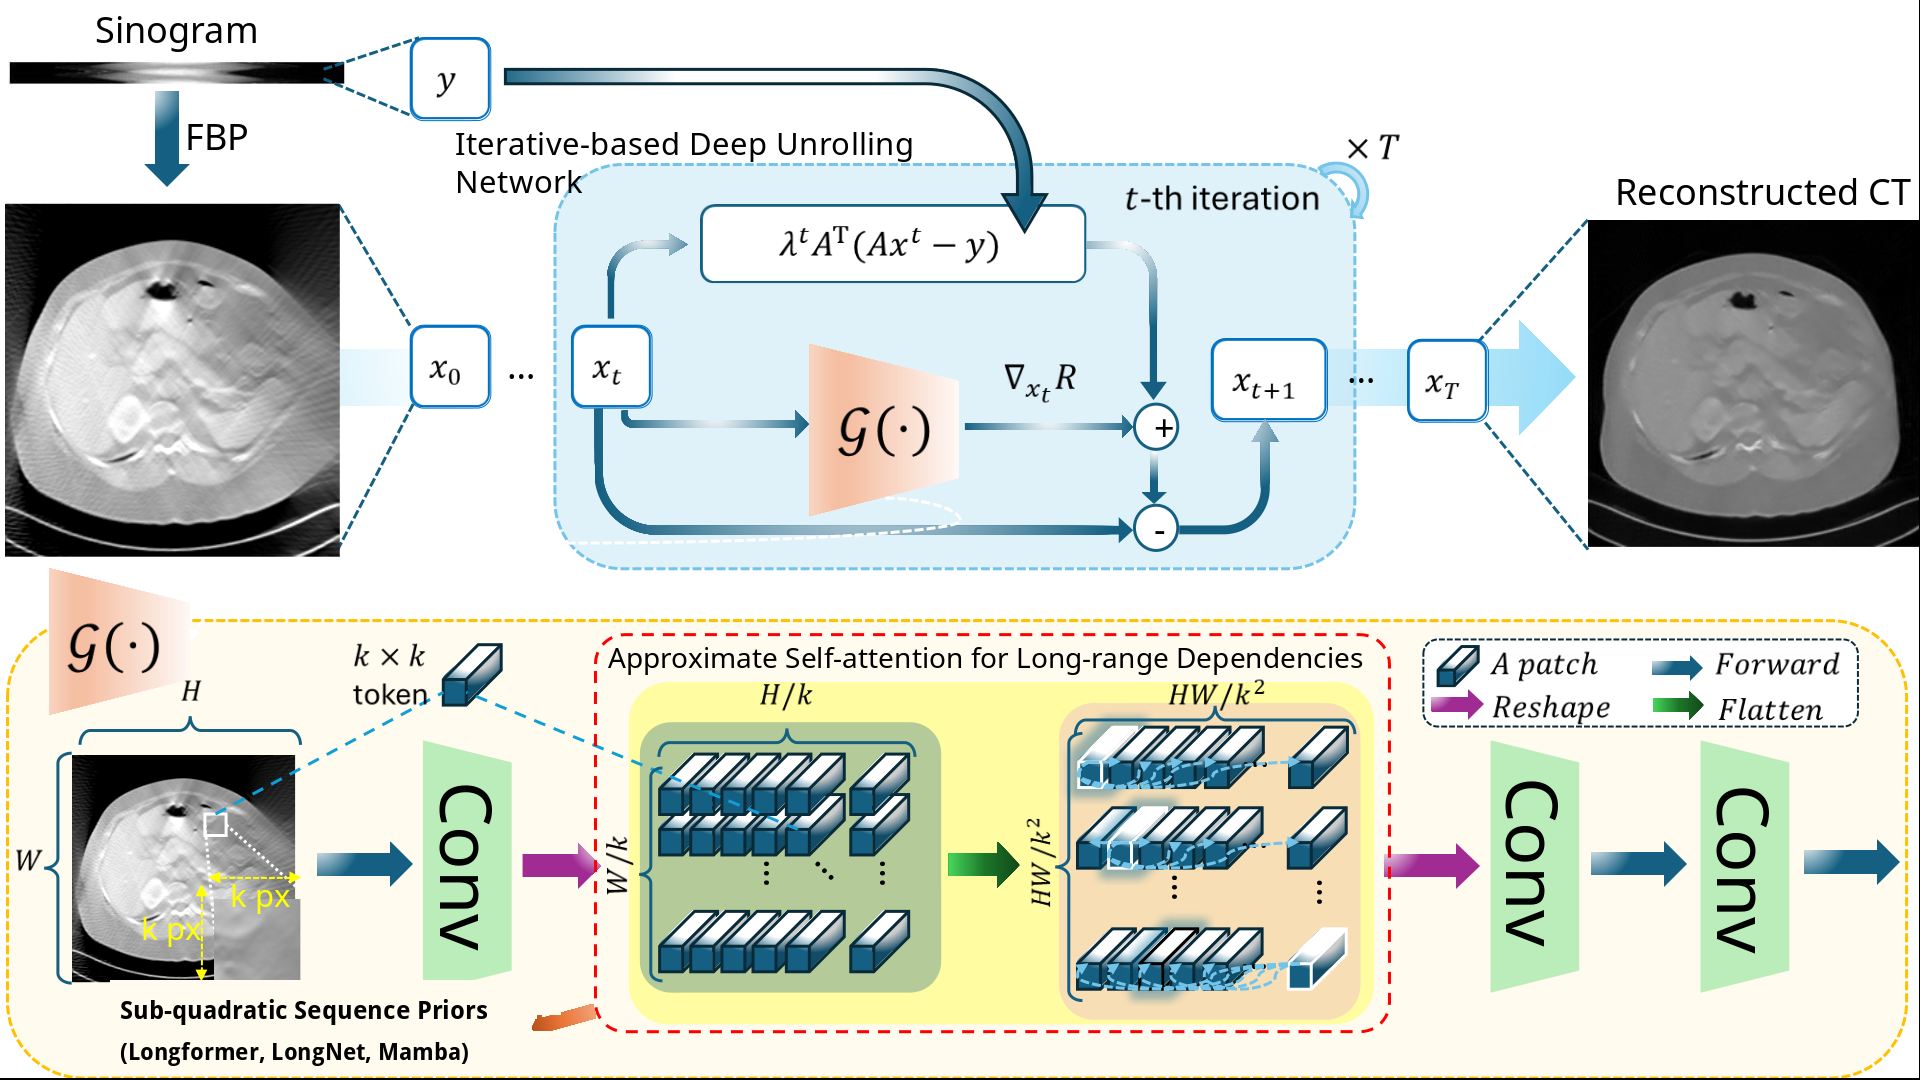
\includegraphics[width=\textwidth]{figures/methodology.png}
\caption{Architectural overview of the deep unfolding framework with long-sequence regularization priors. Top: The $T$-stage iterative unrolling network ($t \in \{0, \dots, T-1\}$, corresponding to stage $k$ in text) unrolls regularized gradient descent, alternating between tomographic data consistency via analytical backprojection ($\lambda^t A^T(A x^t - y)$) and a learned neural regularizer $\mathcal{G}(x_t)$ producing residual update $\nabla_{x_t} R$. Bottom: Detailed structure of the long-sequence regularizer $\mathcal{G}(\cdot)$. The intermediate CT estimate ($H \times W$) is tokenized into non-overlapping $p \times p$ patches to form a sequence of length $HW/p^2$, processed through sub-quadratic sequence mechanisms (LongNet, Longformer, Mamba) to capture long-range streak dependencies across the tomographic slice, and decoded back to image space via convolutional layers.}
\label{fig:methodology}
\end{figure}

The complete reconstruction pipeline and internal prior architecture are illustrated in Fig.~\ref{fig:methodology}. All baseline networks inherit the unrolling structure of LEARN with $K = 14$ cascading stages (corresponding to $T = 14$ iterations in Fig.~\ref{fig:methodology}, with unrolling stage index $k \equiv t$). 

\subsection{Regularization Prior Block Formulation}
\label{sec:reg_block}

As depicted in Fig.~\ref{fig:methodology}, each unrolling stage $k \in \{0, \dots, K-1\}$ computes the learned regularization update $\mathcal{R}_{\theta^{(k)}}(x^{(k)})$ through a structured sandwich architecture comprising an initial spatial convolution, fine-grained patch tokenization, a sub-quadratic sequence engine, inverse spatial folding, and dual convolutional decoding:
\begin{align}
z^{(k)} &= \operatorname{ReLU}\left(\operatorname{Conv}_1\left(x^{(k)}\right)\right), \quad z^{(k)} \in \mathbb{R}^{B \times C \times H \times W}, \label{eq:reg_conv1} \\
Z^{(k)} &= \mathcal{T}_{p \times p}\left(z^{(k)}\right), \quad Z^{(k)} \in \mathbb{R}^{B \times N \times d}, \label{eq:reg_unfold} \\
Z'^{(k)} &= \operatorname{SequenceEngine}\left(Z^{(k)}\right), \quad Z'^{(k)} \in \mathbb{R}^{B \times N \times d}, \label{eq:reg_engine} \\
z'^{(k)} &= \mathcal{T}_{p \times p}^{-1}\left(Z'^{(k)}\right), \quad z'^{(k)} \in \mathbb{R}^{B \times C \times H \times W}, \label{eq:reg_fold} \\
\mathcal{R}_{\theta^{(k)}}\left(x^{(k)}\right) &= \operatorname{Conv}_3\left(\operatorname{ReLU}\left(\operatorname{Conv}_2\left(z'^{(k)}\right)\right)\right), \quad \mathcal{R}_{\theta^{(k)}} \in \mathbb{R}^{B \times 1 \times H \times W}, \label{eq:reg_conv3}
\end{align}
where $\operatorname{Conv}_1$ and $\operatorname{Conv}_2$ operate with kernel size $5 \times 5$ and $C = 48$ intermediate feature channels, while $\operatorname{Conv}_3$ projects the feature map back to a single image channel. The spatial tokenization operator $\mathcal{T}_{p \times p}$ partitions the feature tensor into non-overlapping $p \times p$ patches ($p = 2$), flattening local spatial features across channels to construct an embedding dimension of $d = C \cdot p^2 = 48 \times 2^2 = 192$. On the $H \times W = 256 \times 256$ discretization grid, this yields a sequence of:
\begin{equation}
N = \frac{H}{p} \times \frac{W}{p} = \frac{256}{2} \times \frac{256}{2} = 16,384 \text{ tokens}.
\end{equation}
This fine patch scale ($p = 2$) prevents the blurring of delicate micro-structures caused by coarse patching, while the operator $\operatorname{SequenceEngine}(\cdot)$ captures long-range streak correlations with sub-quadratic complexity.

\subsection{LEARN\_Longformer: Sliding Window with Global Anchors}
Longformer \cite{beltagy2020longformer} substitutes the dense $\mathcal{O}(N^2)$ attention matrix with a hybrid sparse attention pattern. For token sequence $Z \in \mathbb{R}^{N \times d}$ across $H = 6$ attention heads (head dimension $d_h = 32$) and 12 attention layers, query, key, and value representations are $Q, K, V \in \mathbb{R}^{N \times d_h}$. The hybrid attention score matrix $S \in \mathbb{R}^{N \times N}$ is formulated as:
\begin{equation}
S_{i, j} = \begin{cases} 
\frac{Q_i K_j^T}{\sqrt{d_h}}, & |i - j| \leq \frac{w}{2} \text{ or } i \in \mathcal{G} \text{ or } j \in \mathcal{G}, \\ 
-\infty, & \text{otherwise}, 
\end{cases}
\end{equation}
where $w = 256$ is the sliding window width, and $\mathcal{G}$ represents the subset of $|\mathcal{G}| = 50$ global anchor tokens uniformly spaced across the sequence ($i \in \{0, \lfloor \frac{N-1}{|\mathcal{G}|-1} \rfloor, \dots, N-1\}$). The normalized self-attention output for each head is then given by:
\begin{equation}
Z' = \text{Softmax}(S) V.
\end{equation}
The computational complexity scales as $\mathcal{O}(N \cdot (w + |\mathcal{G}|))$, which is strictly linear with respect to sequence length $N$. In tomographic reconstruction, the localized window enforces spatial contiguity to preserve high-contrast bone edges, while global tokens facilitate long-range streak cancellation across distant image coordinates.

\subsection{LEARN\_LongNet: Multi-Scale Exponentially Dilated Attention}
LongNet \cite{ding2023longnet} replaces standard attention with segment-based dilated attention. The token sequence $N = 16,384$ is partitioned into $N / w = 1,024$ non-overlapping segments of length $w = 16$ across $H = 4$ attention heads ($d_h = 48$). Prior to attention calculation, query and key vectors are $\ell_2$-normalized across the channel dimension to enforce numerical stability:
\begin{equation}
\hat{Q} = \frac{Q}{\|Q\|_2}, \quad \hat{K} = \frac{K}{\|K\|_2}.
\end{equation}
For segment $s \in \{1, \dots, N / w\}$ with dilation stride $r$ ($r = 1$ in the baseline regularizer), the dilated attention output is computed as:
\begin{equation}
O_s = \text{Softmax}\left( \frac{\hat{Q}_s \hat{K}_s^T}{\sqrt{d_h}} \right) V_s,
\end{equation}
and the aggregated representations are projected back to the hidden dimension via linear map $W_O \in \mathbb{R}^{d \times d}$:
\begin{equation}
O = \text{Concat}(O_1, \dots, O_{N/w}) W_O.
\end{equation}
In general multi-scale LongNet architectures, outputs from multiple dilation patterns $\{ (w_m, r_m) \}_{m=1}^{M}$ are dynamically aggregated via learnable weights $\sum_{m=1}^{M} \beta_m O^{(m)}$ ($\sum_m \beta_m = 1$), maintaining sub-quadratic complexity $\mathcal{O}(N \cdot \sum_m \frac{w_m}{r_m})$ while capturing heterogeneous spatial frequency bands of CT streak artifacts.

\subsection{LEARN\_Mamba: Selective State-Space Sequential Priors}
Mamba \cite{gu2023mamba} is built upon continuous Structured State Space Sequence Models (S4):
\begin{align}
h'(t) &= A h(t) + B x(t), \\
y(t) &= C h(t) + D x(t).
\end{align}
In Mamba, input-dependent selectivity is introduced by parameterizing $B, C,$ and the discretization timescale $\Delta$ as dynamic linear projections of token $x_t \in \mathbb{R}^{192}$ across $H = 4$ state heads:
\begin{equation}
B_t = W_B x_t, \quad C_t = W_C x_t, \quad \Delta_t = \text{Softplus}(W_\Delta x_t + b_\Delta).
\end{equation}
Discretized using the Zero-Order Hold (ZOH) rule, the system operates as a linear recurrence:
\begin{align}
h_t &= \bar{A}_t h_{t-1} + \bar{B}_t x_t, \quad \bar{A}_t = \exp(\Delta_t A), \quad \bar{B}_t = (\Delta_t A)^{-1}(\exp(\Delta_t A) - I) \Delta_t B_t, \\
y_t &= C_t h_t + D x_t,
\end{align}
where $D \in \mathbb{R}^{d}$ is a learnable direct feedthrough parameter, and the continuous state transition matrix is parameterized via a structured diagonal matrix $A = -\exp(\Theta_A)$ ($\Theta_A \in \mathbb{R}^{d \times N_{\text{state}}}$, with state dimension $N_{\text{state}} = 16$) to strictly enforce $\text{Re}(\lambda_i(A)) < 0$, guaranteeing Bounded-Input Bounded-Output (BIBO) stability while computing recurrences in linear time. For 2D CT images, token grids are serialized into 1D sequences via row-major raster scanning and solved via hardware-aware associative parallel scan in $\mathcal{O}(N)$ linear time.

\section{Experimental Benchmark and Analysis}
\label{sec:experiments}

\subsection{Experimental Setup}
\noindent \textbf{Clinical Dataset:} We utilize the clinical Low-Dose CT (LDCT) Grand Challenge dataset provided by the Mayo Clinic \cite{mccollough2016low}. The dataset contains 10 anonymous patient examinations with normal-dose reference scans ($3\text{ mm}$ slice thickness). Following established protocols, 1,920 slices from 8 patients (\texttt{L067}, \texttt{L096}, \texttt{L109}, \texttt{L143}, \texttt{L192}, \texttt{L286}, \texttt{L291}, \texttt{L506}) form the training set, 244 slices from patient \texttt{L333} form the validation set, and 214 slices from patient \texttt{L310} serve as the independent blind test set. Target slices are standardized to $256 \times 256$ resolution.

\noindent \textbf{Fan-Beam Geometry Simulation:} Projection data are simulated using ASTRA-toolbox and ODL under clinical Fan-Beam geometry matching Siemens Somatom CT systems:
\begin{itemize}
    \item Source-to-isocenter distance: $D_{\text{SO}} = 600\text{ mm}$, isocenter-to-detector distance: $D_{\text{OD}} = 290\text{ mm}$ ($D_{\text{SD}} = 890\text{ mm}$).
    \item Detector array: 512 curved detector channels spanning $[-480\text{ mm}, 480\text{ mm}]$ (fan half-angle $\gamma_m \approx 28.3^\circ$).
    \item Projection views: 64 views sampled uniformly across the limited angular span.
    \item \textbf{Moderate LA-CT ($120^\circ$):} $\theta \in [-60^\circ, +60^\circ]$ (angular step $\Delta\theta \approx 1.875^\circ$).
    \item \textbf{Severe LA-CT ($90^\circ$):} $\theta \in [-45^\circ, +45^\circ]$ (angular step $\Delta\theta \approx 1.406^\circ$, missing $270^\circ$ angular void).
\end{itemize}
Simulations are computed on a $512 \times 512$ physical field-of-view ($[-200\text{ mm}, 200\text{ mm}]$) and downsampled to $256 \times 256$.

\noindent \textbf{Training and Implementation Details:} All unrolling networks are implemented with $K = 14$ stages and trained on NVIDIA A100 GPUs (40GB VRAM). We employ the Adam optimizer with initial learning rate $1 \times 10^{-4}$ and CosineAnnealingLR decay down to $1 \times 10^{-5}$ across 50 epochs (batch size 1, Mean Squared Error loss). Evaluation is conducted on the unseen test set (Patient \texttt{L310}, 214 slices) using Peak Signal-to-Noise Ratio (PSNR in dB), Structural Similarity Index (SSIM), Root Mean Square Error (RMSE), and average inference latency per slice.

\subsection{Quantitative Benchmark Results}

\begin{table}[t]
\centering
\caption{Quantitative reconstruction benchmark under moderate limited-angle geometry ($120^\circ$, 64 views) on the Mayo Clinic LDCT test set (Patient \texttt{L310}, 214 slices). All deep unfolding models operate with $K = 14$ stages and $N = 16,384$ tokens. Latency denotes average GPU inference time per $256 \times 256$ slice on an NVIDIA A100. Best baseline results are in \textbf{bold}, second-best are \underline{underlined}.}
\label{tab:benchmark_120}
\begin{tabular}{lccccc}
\toprule
\textbf{Method / Architecture} & \textbf{Params (M)} & \textbf{PSNR (dB)} $\uparrow$ & \textbf{SSIM} $\uparrow$ & \textbf{RMSE} $\downarrow$ & \textbf{Latency} $\downarrow$ \\
\midrule
Analytical FBP (Ram-Lak) & -- & 17.89 & 0.4984 & 0.1145 & $< 5\text{ ms}$ \\
DuDoTrans \cite{wang2022dudotrans} & 0.13 & 25.15 & 0.7447 & 0.0650 & $\approx 15\text{ ms}$ \\
LEARN (Original CNN) \cite{chen2018learn} & 0.84 & \underline{32.29} & \textbf{0.9383} & \underline{0.0246} & $\approx 20\text{ ms}$ \\
LEARN\_Mamba \cite{gu2023mamba} & 2.9 & 26.32 & 0.7468 & 0.0493 & $\approx 12\text{ ms}$ \\
LEARN\_LongNet \cite{ding2023longnet} & 2.4 & 31.62 & 0.8991 & 0.0270 & $\approx 28\text{ ms}$ \\
LEARN\_Longformer \cite{beltagy2020longformer} & 4.0 & \textbf{33.10} & \underline{0.9237} & \textbf{0.0224} & $\approx 45\text{ ms}$ \\
\bottomrule
\end{tabular}
\end{table}

\begin{table}[t]
\centering
\caption{Quantitative reconstruction benchmark under severe limited-angle geometry ($90^\circ$, 64 views, missing $270^\circ$ angular void) on the Mayo Clinic LDCT test set (Patient \texttt{L310}, 214 slices). Best baseline results are in \textbf{bold}, second-best are \underline{underlined}.}
\label{tab:benchmark_90}
\begin{tabular}{lccccc}
\toprule
\textbf{Method / Architecture} & \textbf{Params (M)} & \textbf{PSNR (dB)} $\uparrow$ & \textbf{SSIM} $\uparrow$ & \textbf{RMSE} $\downarrow$ & \textbf{Latency} $\downarrow$ \\
\midrule
Analytical FBP (Ram-Lak) & -- & 15.20 & 0.4120 & 0.1450 & $< 5\text{ ms}$ \\
DuDoTrans \cite{wang2022dudotrans} & 0.13 & \underline{21.81} & \underline{0.6738} & \underline{0.0842} & $\approx 15\text{ ms}$ \\
LEARN (Original CNN) \cite{chen2018learn} & 0.84 & \textbf{28.03} & \textbf{0.8793} & \textbf{0.0411} & $\approx 20\text{ ms}$ \\
LEARN\_Mamba \cite{gu2023mamba} & 2.9 & 18.76 & 0.4292 & 0.1129 & $\approx 12\text{ ms}$ \\
LEARN\_LongNet \cite{ding2023longnet} & 2.4 & 19.19 & 0.5876 & 0.1058 & $\approx 28\text{ ms}$ \\
LEARN\_Longformer \cite{beltagy2020longformer} & 4.0 & 19.16 & 0.6097 & 0.1055 & $\approx 45\text{ ms}$ \\
\bottomrule
\end{tabular}
\end{table}

The primary quantitative comparisons on Patient \texttt{L310} under moderate ($120^\circ$) and severe ($90^\circ$) scanning regimes are summarized in Table~\ref{tab:benchmark_120} and Table~\ref{tab:benchmark_90}, respectively. Several critical findings emerge:

\noindent \textbf{1. Superiority of LEARN\_Longformer at $120^\circ$ and Comparison with Canonical CNN LEARN:} 
LEARN\_Longformer achieves the highest reconstruction accuracy among all sequence-based architectures, delivering \textbf{33.10 dB PSNR} and the lowest RMSE of \textbf{0.0224} at $120^\circ$. Compared to the canonical CNN-based LEARN baseline (32.29 dB PSNR, 0.0246 RMSE), LEARN\_Longformer yields a $+0.81$ dB improvement in PSNR and reduces reconstruction error energy (RMSE) by $8.9\%$. This performance margin highlights the clear advantage of non-local sequence modeling over purely localized convolutions. Standard LEARN relies on 3-layer $5 \times 5$ convolutions whose cumulative receptive field per stage is restricted to $13 \times 13$ pixels, rendering it incapable of resolving extensive streak trajectories that traverse the entire $256 \times 256$ field of view. In contrast, LEARN\_Longformer combines sliding-window attention ($w = 256$) with $|\mathcal{G}| = 50$ global anchor tokens uniformly spaced across the 16,384-token sequence, enabling long-range streak cancellation across distant anatomical regions. While standard LEARN attains a higher SSIM (0.9383 vs. 0.9237) due to the strong local smoothing prior of convolutional filters on homogeneous soft tissues, its peak signal accuracy remains bounded by its restricted spatial horizon.

\noindent \textbf{2. Performance of Deep Unfolding vs. Dual-Domain Feedforward Processing (DuDoTrans):}
At $120^\circ$, all iterative deep unfolding networks dramatically outperform the feedforward dual-domain transformer DuDoTrans (25.15 dB PSNR, 0.7447 SSIM, 0.0650 RMSE). LEARN\_Longformer surpasses DuDoTrans by $+7.95$ dB PSNR, $+0.1790$ SSIM, and achieves a nearly $3\times$ reduction in RMSE ($0.0224$ vs. $0.0650$). Even LEARN\_LongNet (31.62 dB) and canonical CNN LEARN (32.29 dB) outperform DuDoTrans by more than 6.4 dB. This contrast underscores the essential role of iterative tomographic data consistency: while DuDoTrans relies on sinogram transformer inpainting followed by a single-pass filtered backprojection and an image enhancement module, deep unfolding networks enforce physical projection fidelity $\alpha^{(k)} A^T(A x^{(k)} - y)$ across 14 cascaded stages, systematically eliminating non-physical hallucinations.

\noindent \textbf{3. The Inpainting Resilience of DuDoTrans Under Severe $90^\circ$ Truncation:}
Under severe $90^\circ$ truncation (where $270^\circ$ of projection data is missing), a remarkable domain-level insight emerges: DuDoTrans attains \textbf{21.81 dB PSNR} and \textbf{0.6738 SSIM}, markedly outperforming all three 1st-order long-sequence unrolling models (LEARN\_Longformer: 19.16 dB / 0.6097, LEARN\_LongNet: 19.19 dB / 0.5876, and LEARN\_Mamba: 18.76 dB / 0.4292). This highlights a fundamental distinction between projection-domain and image-domain restoration: under a massive $270^\circ$ angular void, the image-domain data fidelity gradient $\alpha A^T(Ax - y)$ in first-order unrolling largely vanishes across the missing frequency cone $\Omega_{\text{missing}}$, creating severe optimization stalling in image space. Conversely, sinogram projections are continuous sinusoidal curves governed by Helgason-Ludwig consistency conditions \cite{kak2001principles}. By performing self-attention directly in the sinogram domain prior to backprojection, DuDoTrans effectively interpolates missing projection paths, providing a structurally coherent input that avoids the frequency blackout suffered by pure image-domain gradient descent.

\noindent \textbf{4. Locality Robustness of Compact Convolutions in LEARN at $90^\circ$:}
Under $90^\circ$ scanning, canonical CNN-based LEARN maintains \textbf{28.03 dB PSNR} and \textbf{0.8793 SSIM}. With only 0.84M parameters and strictly localized $5 \times 5$ spatial kernels, the 3-layer convolutional regularizer acts as a conservative, translation-equivariant denoiser that avoids optimization divergence. In contrast, 16,384-token sequence models (2.4M--4.0M parameters) possess vast representational degrees of freedom that become unconstrained when physical data consistency gradients provide zero feedback across $50\%$ of the Fourier domain, causing the unrolled optimization trajectory to plateau around $19.2$ dB.

\noindent \textbf{5. Vulnerability of Mamba Under 2D Anisotropic Truncation:}
While LEARN\_Mamba achieves rapid inference ($\approx 12\text{ ms}$/slice) and an adequate PSNR of 26.32 dB at $120^\circ$, its performance drops sharply to \textbf{18.76 dB PSNR} and \textbf{0.4292 SSIM} at $90^\circ$, yielding an SSIM barely superior to analytical FBP ($0.4120$). This reveals an essential theoretical insight: Mamba's 1D causal scanning along flattened rows imposes an artificial 1D directional inductive bias. In limited-angle tomography, the missing-wedge void is intrinsically 2D and anisotropic. Serializing 2D feature grids into 1D sequences breaks vertical column continuity, preventing the 1D state transition from propagating correlations orthogonal to its scan line. Furthermore, in deep 14-stage unrolling, Mamba reached peak validation performance at Epoch 17 (PSNR 27.66 dB, SSIM 0.7373); continuing training beyond Epoch 20 suffered from numerical gradient instability due to the absence of spectrum damping on the ill-conditioned Hessian.

\subsection{Qualitative Visual Comparison}

\begin{figure}[t]
\centering
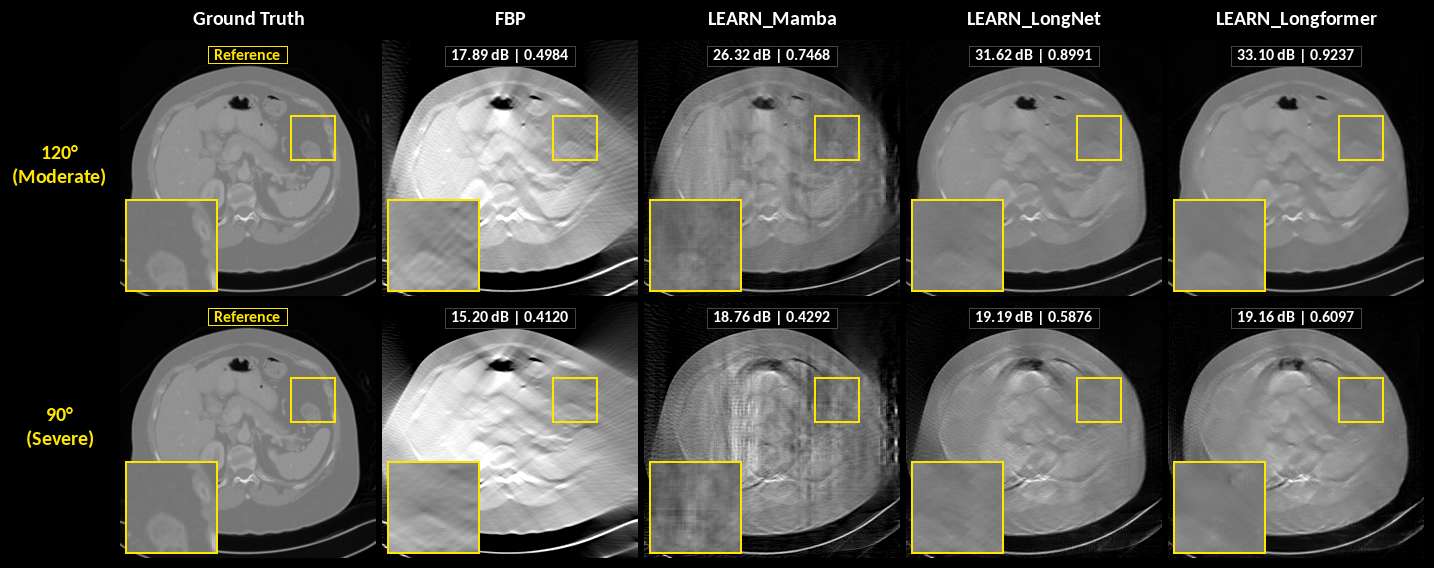
\includegraphics[width=\textwidth]{figures/visual_comparison_roi.png}
\caption{Multi-regime visual comparison of reconstructed CT slices on the Mayo Clinic LDCT benchmark (Patient \texttt{L310}, Slice 050). Top row: Moderate $120^\circ$ scanning ($64$ views). Bottom row: Severe $90^\circ$ scanning ($64$ views, $270^\circ$ missing-wedge void). Columns illustrate analytical FBP, canonical CNN-based LEARN, feedforward dual-domain DuDoTrans, and sequence-based unrolling models (LEARN\_Mamba, LEARN\_LongNet, LEARN\_Longformer). Metrics stamped above each panel denote the overall test-set mean (PSNR [dB] | SSIM) across all 214 slices of Patient \texttt{L310} for baseline reference (individual Slice 050 metrics for Longformer are 33.73 dB / 0.9107 at $120^\circ$). Yellow bounding boxes denote an anatomical Region of Interest (ROI) spanning the lateral rib boundary and peripheral soft-tissue interfaces, magnified by $3\times$ in the bottom-left insets. Quantitatively, LEARN\_Longformer achieves superior boundary fidelity and tissue preservation at $120^\circ$, while under extreme $90^\circ$ truncation, canonical LEARN exhibits conservative smoothing while sequence models suffer from the unconstrained ill-conditioned null space.}
\label{fig:visual_comparison_roi}
\end{figure}

Fig.~\ref{fig:visual_comparison_roi} presents a comprehensive visual benchmark across both moderate ($120^\circ$) and severe ($90^\circ$) scanning geometries, with magnified insets highlighting structural recovery:
\begin{itemize}
    \item \textbf{Analytical FBP} displays intense, high-amplitude streak artifacts traversing the entire field of view, completely destroying soft-tissue contrast and causing severe shadow distortion.
    \item \textbf{LEARN (Original CNN)} achieves high noise suppression due to its local convolutional smoothing prior, but its restricted $13 \times 13$ effective receptive field leaves fine, high-frequency periodic ripple streaks visible in the magnified ROI at $120^\circ$. At $90^\circ$, it retains conservative stability ($0.8793$ SSIM) while suffering noticeable edge blurring across anatomical interfaces.
    \item \textbf{DuDoTrans} reduces coarse streaking via sinogram transformer inpainting, but the absence of iterative projection data consistency produces prominent residual shading artifacts and structural attenuation in both scanning regimes.
    \item \textbf{LEARN\_Mamba} mitigates coarse streaks at $120^\circ$, but the magnified ROI reveals significant low-frequency shading artifacts and blurred bone interfaces. At $90^\circ$, Mamba collapses into severe geometric deformation, failing to separate the rib boundary from surrounding parenchyma due to 1D directional serialization.
    \item \textbf{LEARN\_LongNet} restores major organ contours and substantially suppresses peripheral streaks via its multi-scale dilated receptive field, though subtle boundary blur remains visible in the zoomed inset.
    \item \textbf{LEARN\_Longformer} delivers the highest structural fidelity at $120^\circ$, restoring crisp rib margins, uniform abdominal soft-tissue density, and eliminating streak contamination across the reconstructed slice. Under $90^\circ$, it retains the highest SSIM ($0.6097$) among the sequence-based unrolling architectures, though bounded by canonical CNN LEARN ($0.8793$) and dual-domain DuDoTrans ($0.6738$), with residual edge elongation persisting due to the fundamental missing wedge.
\end{itemize}

\begin{figure}[t]
\centering
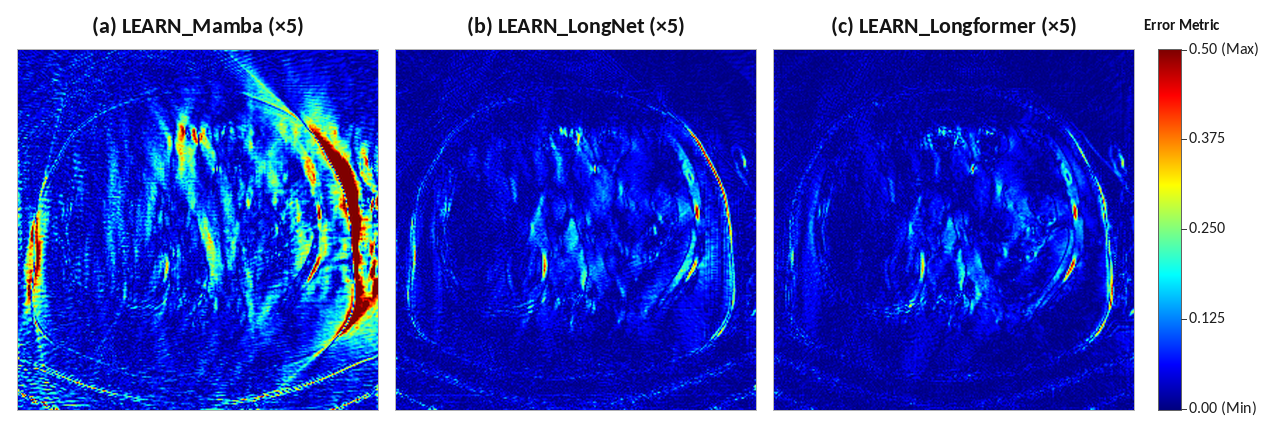
\includegraphics[width=\textwidth]{figures/residual_error_maps.png}
\caption{Residual absolute error maps $|x_{\text{recon}} - x^*|$ scaled by a factor of 5 using the 'jet' colormap under moderate $120^\circ$ scanning (Patient \texttt{L310}, Slice 050): (a) LEARN\_Mamba, (b) LEARN\_LongNet, and (c) LEARN\_Longformer. Blue indicates near-zero error energy, while red denotes severe discrepancy. LEARN\_Longformer exhibits near-uniform blue background, verifying its superior artifact elimination across both streak pathways and soft-tissue parenchyma.}
\label{fig:error_maps}
\end{figure}

\begin{figure}[t]
\centering
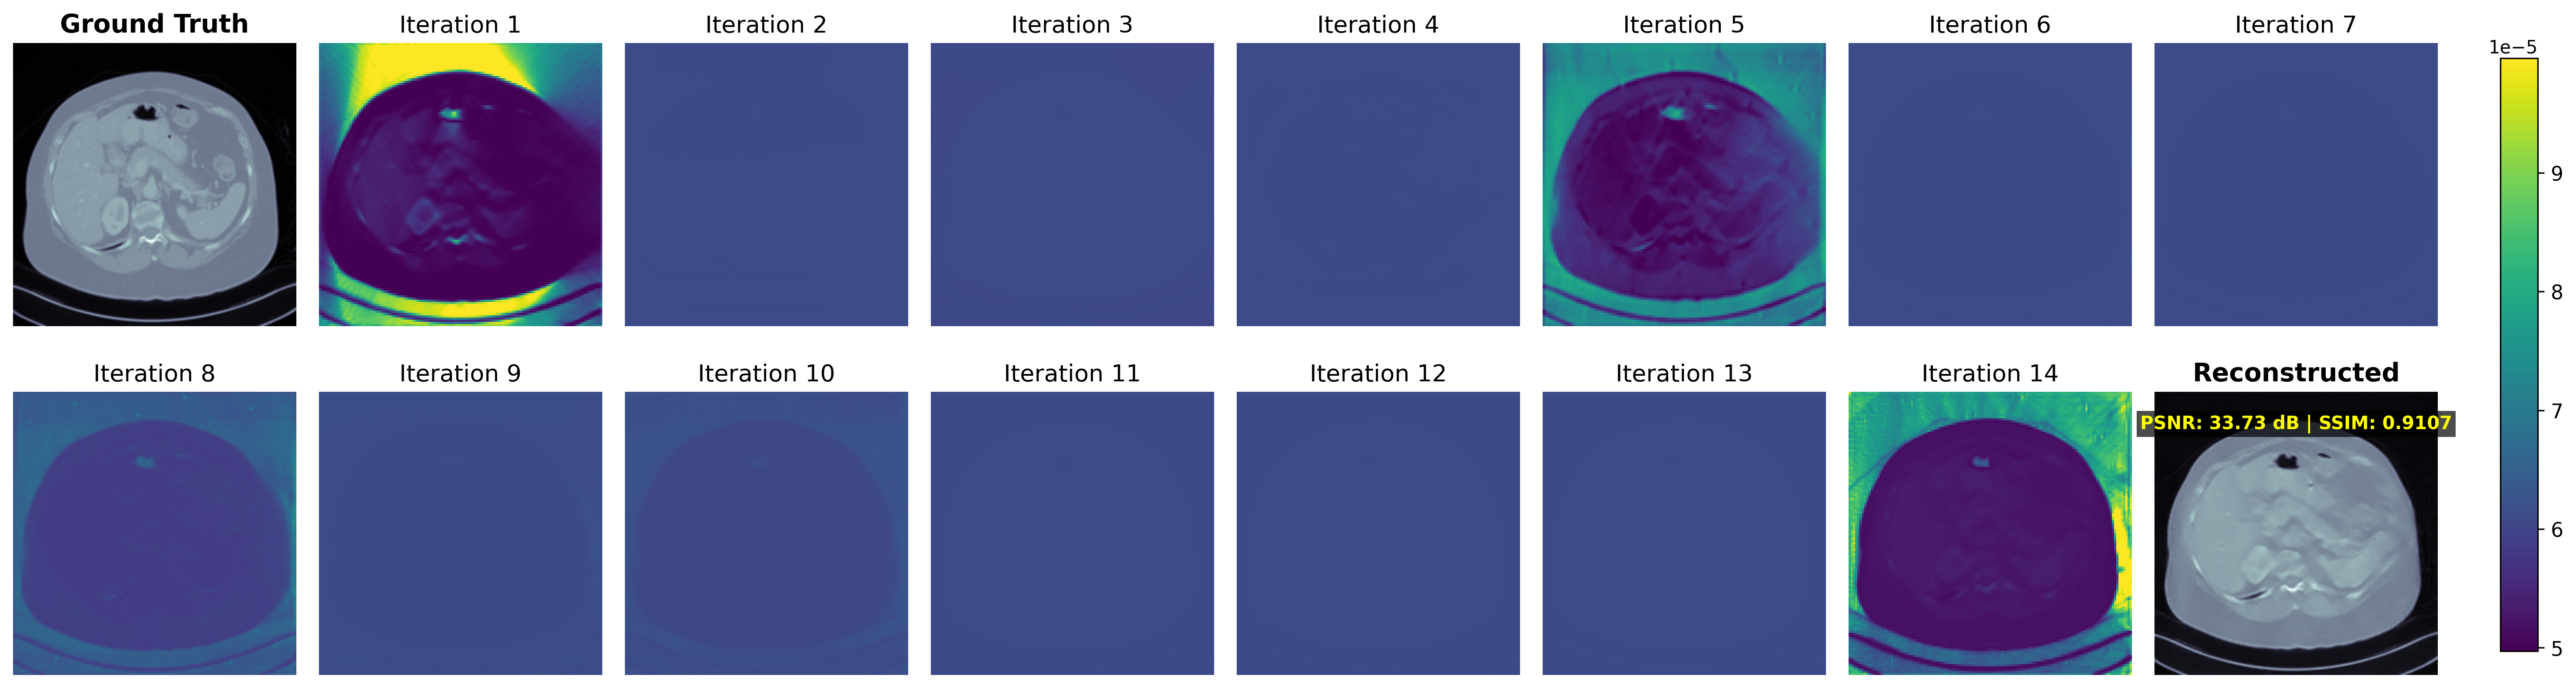
\includegraphics[width=\textwidth]{figures/longformer_attn_evolution_120deg_slice050.png}
\caption{Evolution of Longformer self-attention maps across $K = 14$ deep unrolling iterations under moderate limited-angle scanning ($120^\circ$, 64 views, Patient \texttt{L310}, Slice 050). Each panel visualizes the dynamic attention distribution of the global anchor token reshaped to $128 \times 128$ spatial resolution. In early iterations ($t=1 \to 5$), attention concentrates heavily along the peripheral boundaries and high-frequency streak trajectory interfaces. In intermediate and final iterations ($t=6 \to 14$), attention shifts dynamically to refine soft-tissue contrast and internal organ contours, achieving high-fidelity reconstruction ($33.73\text{ dB}$ PSNR, $0.9107$ SSIM).}
\label{fig:attn_evolution}
\end{figure}

The bottom row of Fig.~\ref{fig:visual_comparison_roi} further illustrates the severe $90^\circ$ regime, where structural distortion and edge blurring remain pronounced across all baselines due to the massive $270^\circ$ missing-wedge void, directly corroborating our quantitative benchmark. 

To evaluate residual discrepancy across the slice, the error maps in Fig.~\ref{fig:error_maps} visually corroborate the superior streak suppression of LEARN\_Longformer, which yields a predominantly uniform low-energy blue distribution compared to the noticeable residual error concentrations observed in LEARN\_Mamba and LEARN\_LongNet.

Finally, to elucidate the internal representational dynamics through which Longformer suppresses anisotropic streak artifacts across the iterative unrolling trajectory, Fig.~\ref{fig:attn_evolution} illustrates the spatial evolution of the global anchor attention weights across all $K=14$ unrolling stages. In the initial iterations ($t=1\to 2$), attention energy is intensely concentrated on the peripheral boundaries and high-frequency streak trajectories where back-projection gradient discrepancies $\alpha A^T(Ax - y)$ are most acute. Over intermediate iterations ($t=3\to 10$), the attention distribution rapidly diffuses to a highly sparse, uniform baseline across the 16,384 tokens ($\sim 6.1 \times 10^{-5}$, reflected in the uniform blue background tone) while intermittently activating localized tissue anchors (e.g., at $t=5$ and $t=8$) to restore soft-tissue homogeneity across the missing-wedge void. In the final stages ($t=11\to 14$), attention reconcentrates along structural boundaries to perform fine-grained sharpening, validating the interpretability and physical grounding of Longformer's combined sliding-window and global token architecture.

\section{Discussion and Future Directions}
\label{sec:discussion}

The empirical findings from our benchmark provide several foundational principles for the design of physics-guided iterative reconstruction architectures:

\subsection{Geometric Duality: Sparse-View vs. Limited-Angle Tomography}
A critical insight emerges when comparing our findings in limited-angle tomography with recent investigations in sparse-view CT reconstruction \cite{bui2026mva}. In sparse-view acquisition, projection angles are uniformly distributed over the entire angular circle $[0, 2\pi]$ (e.g., 32 or 64 evenly spaced views). Under this isotropic geometry, missing information manifests as dense radial sampling gaps, producing radially distributed, symmetric streak artifacts. In that regime, landmark-based approximations such as Nystr{\"o}mformer \cite{xiong2021nystromformer} excel because uniformly sampled landmarks effectively capture the isotropic spatial statistics across the field of view \cite{bui2026mva}.

In sharp contrast, limited-angle CT introduces an intrinsically \textit{anisotropic} missing-wedge cone $\Omega_{\text{missing}}$ in Fourier frequency space. The resulting artifacts do not radiate symmetrically; instead, they form intense directional streaks aligned with the tangent of the missing angular boundaries, accompanied by severe edge elongation and loss of surface gradients perpendicular to the missing rays. Under this directional degradation, \textbf{Longformer}'s inductive bias is uniquely matched to the underlying physics: its dense sliding window ($w = 256$) preserves local edge continuity and tissue contrast along the well-sampled angular trajectories, while its sparse global anchors ($|\mathcal{G}| = 50$) anchor non-local streak cancellation across the entire slice, enabling it to outperform all competing baselines (33.10 dB PSNR).

\subsection{Structural Vulnerability of 1D Causal Scanning}
While selective state-space models like Mamba achieve impressive inference speed ($\approx 12\text{ ms}$/slice with 2.9M parameters), their sequential raster-scan paradigm introduces a severe geometric limitation when applied to 2D inverse problems. By serializing 2D image grids into 1D sequences, horizontal line scanning breaks vertical and diagonal neighborhood topology. When confronting a 2D anisotropic missing wedge (particularly at severe $90^\circ$ scanning), Mamba cannot propagate state transitions across the boundary of the frequency void, resulting in structural collapse and severe low-frequency shading artifacts. For state-space architectures to succeed in tomography, future research must incorporate multi-directional, angle-aware 2D scanning paths or sinogram-guided projection-space routing.

\subsection{Trade-Off Between Architectural Complexity and Clinical Latency}
Our benchmark illuminates clear clinical trade-offs across distinct architectural paradigms:
\begin{itemize}
    \item \textbf{LEARN\_Longformer} (4.0M params, $\approx 45\text{ ms}$ latency) provides the highest diagnostic signal fidelity (33.10 dB PSNR at $120^\circ$) and superior streak elimination, making it ideal for high-precision diagnostic CT where structural sharpness is paramount.
    \item \textbf{LEARN (Original CNN)} (0.84M params, $\approx 20\text{ ms}$ latency) provides a remarkably stable and compact unrolling prior with the highest SSIM (0.9383 at $120^\circ$), but its restricted $5 \times 5$ receptive field prevents it from matching Longformer's peak PSNR and RMSE.
    \item \textbf{LEARN\_LongNet} (2.4M params, $\approx 28\text{ ms}$ latency) achieves an appealing balance between parameter footprint and multi-scale contextual aggregation, delivering 31.62 dB PSNR via dilated attention.
    \item \textbf{DuDoTrans} (0.13M params, $\approx 15\text{ ms}$ latency) features the smallest parameter footprint and rapid execution via feedforward dual-domain transformation, but its lack of iterative data fidelity updates bounds its reconstruction accuracy at $120^\circ$ (25.15 dB).
    \item \textbf{LEARN\_Mamba} (2.9M params, $\approx 12\text{ ms}$ latency) achieves near real-time throughput, but requires architectural adaptation to mitigate its vulnerability to severe angular voids.
\end{itemize}

\subsection{Convergence Ceiling of First-Order Unrolling and Dual-Domain Synergy}
Finally, the convergence plateau observed under severe $90^\circ$ scanning ($\approx 19.2\text{ dB}$ across image-domain long-sequence unrolling models) highlights an intrinsic mathematical limitation of first-order gradient descent. When $50\%$ of the projection angular sweep is missing, the normal operator $A^TA$ possesses a vast null space where gradient steps $\alpha A^T(Ax - y)$ vanish to zero. Purely learned first-order regularizers cannot independently synthesize missing frequency components in the complete absence of physical gradient feedback. 

Crucially, the resilience of \textbf{DuDoTrans} at $90^\circ$ (21.81 dB PSNR / 0.6738 SSIM) provides an indispensable physical lesson: while image-domain gradients stall in the missing Fourier wedge, sinograms are continuous functions governed by smooth projection geometry constraints. Inpainting missing projection views in the sinogram domain before filtered backprojection effectively circumvents the image-space gradient null space. Meanwhile, the stability of canonical CNN LEARN (28.03 dB) demonstrates that compact, translation-equivariant local regularizers avoid the over-parameterization divergence of unconstrained 16,384-token sequence models under zero-gradient conditions. These comparative insights indicate that next-generation reconstruction frameworks should combine dual-domain sinogram inpainting with second-order curvature preconditioning to conquer extreme limited-angle tomography.

\section{Conclusion}
\label{sec:conclusion}

In this paper, we presented a comprehensive empirical benchmark investigating modern sub-quadratic long-sequence modeling mechanisms---Longformer, LongNet, and Mamba---embedded as learnable regularizers within the LEARN deep unfolding framework for limited-angle CT reconstruction, benchmarked against canonical CNN-based deep unfolding (LEARN) and dual-domain transformer architecture (DuDoTrans). Extensive experiments on the clinical Mayo Clinic LDCT dataset across moderate ($120^\circ$) and extreme ($90^\circ$) angular shortages demonstrate that \textbf{LEARN\_Longformer} attains state-of-the-art performance at $120^\circ$ (33.10 dB PSNR, 0.0224 RMSE), outperforming canonical CNN LEARN (+0.81 dB) and DuDoTrans (+7.95 dB), proving that local windowing with sparse global tokens optimally balances local boundary preservation with non-local streak suppression. Furthermore, our analysis reveals the domain advantage of sinogram-space inpainting (DuDoTrans) under extreme $90^\circ$ frequency voids, uncovers the structural vulnerability of 1D state-space models (Mamba) under anisotropic 2D truncation, and identifies the theoretical convergence ceiling of first-order unrolling networks, offering foundational architectural guidelines for medical inverse problems.

\bibliographystyle{splncs04}
\bibliography{refs}

\end{document}
